\mySection{7.4  Drawing Inferences About $\mu$}
%-------------- start slide -------------------------------%{{{ 7.39
\begin{frame}
	% {\S\: 7.4  Drawing Inferences About $\mu$}
\begin{enumerate}
	\item[] Let $Y_1,\cdots,Y_n$ be a random sample from $N(\mu,\sigma^2)$.\\[1em]
	\item[Question] Find a test statistic $\Lambda$ in order to test\qquad $H_0 : \mu = \mu_0$ v.s. $H_1 : \mu \ne \mu_0$.
\vfill
\item[Case I.] $\sigma^2$ is known: \hspace{4em}
	$\displaystyle	\Lambda =  \frac{\overline{Y}-\mu_0}{\sigma/\sqrt{n}}$
\vfill
\item[Case II.] $\sigma^2$ is unknown: \hspace{3em} $\displaystyle \Lambda = \alert{?}$
	\pause \hspace{3em}
	$\displaystyle	\Lambda \stackrel{\alert{?}}{=}  \frac{\overline{Y}-\mu_0}{s/\sqrt{n}}\quad \sim\quad \alert{?}$
\end{enumerate}
\end{frame}
%-------------- end slide -------------------------------%}}}
%-------------- start slide -------------------------------%{{{ 7.40
\begin{frame}{Summary}
\begin{center}
A random sample of size $n$ from \\
a normal distribution $N(\mu,\sigma^2)$\\[2em]
\def\arraystretch{2}
\small
\begin{tabular}{c|c|c}
& $\sigma^2$ known & $\sigma^2$ unknown \\
\hline\hline
Statistic &
$Z = \frac{\overline{Y}-\mu}{\sigma/\sqrt{n}}$ &
$T_{n-1} = \frac{\overline{Y}-\mu}{S/\sqrt{n}}$\\
\hline
Score &
$z = \frac{\overline{y}-\mu}{\sigma/\sqrt{n}}$ &
$t = \frac{\overline{y}-\mu}{s/\sqrt{n}}$\\
\hline
Table & $z_{\alpha}$ & $t_{\alpha,n-1}$ \\
\hline
$100(1-\alpha)\%$ C.I. &
$\left( \bar{y}-z_{\alpha/2}\frac{\sigma}{\sqrt{n}}, \bar{y}+z_{\alpha/2}\frac{\sigma}{\sqrt{n}}\right)$ &
$\left( \bar{y}-t_{\alpha/2,n-1}\frac{s}{\sqrt{n}}, \bar{y}+t_{\alpha/2,n-1}\frac{s}{\sqrt{n}}\right)$ \\
\hline
Test $H_0:\mu=\mu_0$ &
&
\\
$H_1:\mu>\mu_0$ &   Reject $H_0$ if $z\ge z_{\alpha}$
&   Reject $H_0$ if $t\ge t_{\alpha,n-1}$
\\
$H_1:\mu<\mu_0$ &  Reject $H_0$ if $z\le z_{\alpha}$
&  Reject $H_0$ if $t\le t_{\alpha,n-1}$
\\
$H_1:\mu\ne\mu_0$ &  Reject $H_0$ if $|z|\ge z_{\alpha/2}$
&    Reject $H_0$ if $|t|\ge t_{\alpha/2,n-1}$
\\
\hline
\end{tabular}
\end{center}
\end{frame}
%-------------- end slide -------------------------------%}}}
%-------------- start slide -------------------------------%{{{ 7.41
\begin{frame}{Computing $s$ from data}
\begin{enumerate}
	\item[Step 1] $\displaystyle a=\sum_{i=1}^n y_i$
	\item[Step 2.] $\displaystyle b=\sum_{i=1}^n y_i^2$
	\item[Step 3.] $\displaystyle s =\sqrt{\frac{n b-a^2}{n(n-1)} } $
\vfill
\item[Proof.]\[
s^2 = \frac{1}{n-1}\sum_{i=1}^n (y_i-\bar{y})^2  =
\frac{n\left(\sum_{i=1}^n y_i^2\right) -\left(\sum_{i=1}^n y_i \right)^2}{n(n-1)}
\]
\myEnd
\end{enumerate}
\end{frame}
%-------------- end slide -------------------------------%}}}
%-------------- start slide -------------------------------%{{{ 7.42 Case 7.4.1
\begin{frame}
\begin{enumerate}
	\item[Case \small 7.4.1] How far apart are the bat and the insect when the bat first senses that insect is there? \\
	\item[] Or, what is the effective range of a bat's echolocation system?
		\begin{center}
		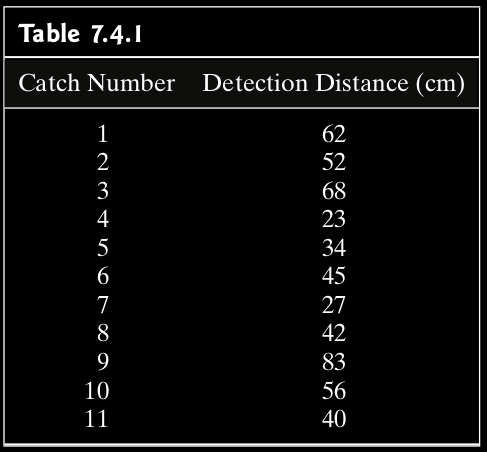
\includegraphics[scale=0.25]{Table_7-4-1-neg.png}
		\end{center}
	\item[] Answer the question by contruct a 95\% C.I.
\vfill
\item[Sol.] ... \myEnd
\end{enumerate}
\end{frame}
%-------------- end slide -------------------------------%}}}
%-------------- start slide -------------------------------%{{{ 1
\begin{frame}[fragile]
	\begin{lstlisting}[language=Python]
# Case7_4_1.py
import numpy as np
import scipy.stats as st


# returns confidence interval of mean
def confIntMean(a, conf=0.95):
    mean, sem, m = np.mean(a), st.sem(a), st.t.ppf((1+conf)/2., len(a)-1)
    return mean - m*sem, mean + m*sem


def main():
    alpha = 5
    data = np.array([62, 52, 68, 23, 34, 45, 27, 42, 83, 56, 40])
    lower, upper = confIntMean(data, 1-alpha/100)
    print("""\

    The {alpha}% confidence interval is ({lower:.2f},{upper:.2f})

        """.format(**locals()))


if __name__ == "__main__":
    main()
	\end{lstlisting}
	\begin{lstlisting}[language=Python]
In [83]: run Case7_4_1.py

    The 95% confidence interval is (36.21,60.51)


	\end{lstlisting}
\end{frame}
%-------------- end slide -------------------------------%}}}

%-------------- start slide -------------------------------%{{{ 7.43
\begin{frame}
	\begin{enumerate}
		\item[Eg. \small 7.4.2] Bank approval rates for inner-city residents v.s. rural ones.\\
		\item[] Approval rate for rural residents is 62\%.\\
		\item[] Do bank treat two groups equally? $\alpha=0.05$
			\begin{center}
				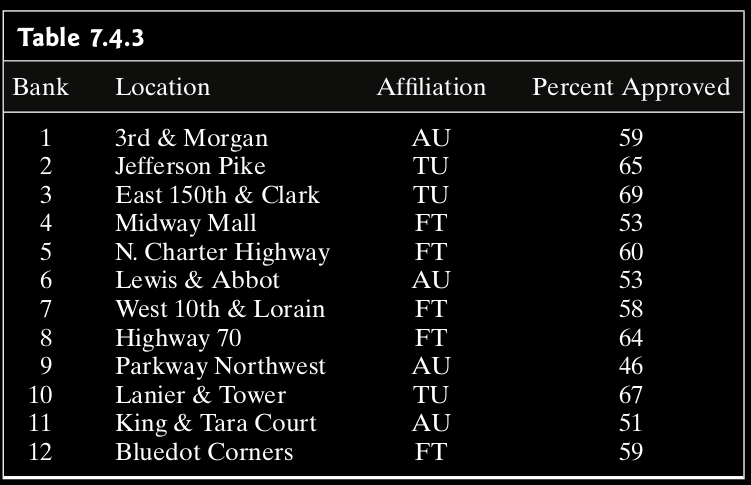
\includegraphics[scale=0.25]{Table_7-4-3-neg.png}
			\end{center}
		\vfill
		\item[Sol.]
			\[
			H_0: \mu = 62\qquad v.s. \qquad H_1: \mu \ne 62.
			\]
	\end{enumerate}
\end{frame}
%-------------- end slide -------------------------------%}}}
%-------------- start slide -------------------------------%{{{ 7.44
\begin{frame}
\centering
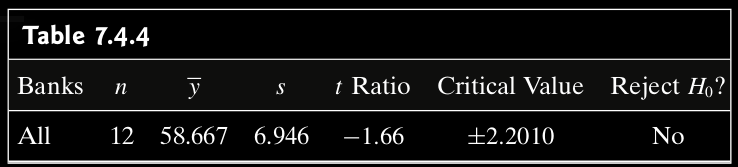
\includegraphics[scale=0.25]{Table_7-4-4-neg.png}
\vfill
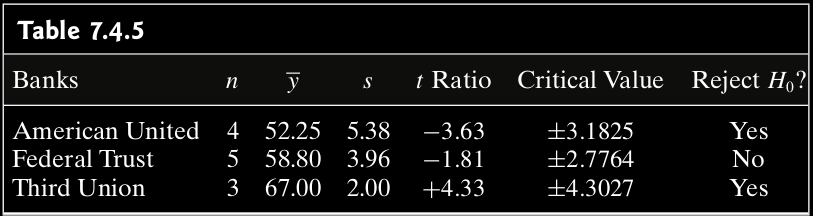
\includegraphics[scale=0.25]{Table_7-4-5-neg.png}
\end{frame}
%-------------- end slide -------------------------------%}}}
%-------------- start slide -------------------------------%{{{ 1 Codes for Eg 7.4.2
\begin{frame}[fragile]
\begin{lstlisting}[language=Python]
# Eg7_4_2.py
import numpy as np
import scipy.stats as st

data = np.array([59, 65, 69, 53, 60, 53, 58, 64, 46, 67,  51, 59])
alpha = 5
mean, sem = np.mean(data), st.sem(data)
n = len(data)
s = sem * np.sqrt(n)
cv = st.t.ppf(1-alpha/200., len(data)-1)
tRatio = (mean-62)/sem


print("""\

      n={n}, sample mean={mean:.3f}, s={s:.3f}, t Ratio={tRatio:.2f}, Critical values={cv:.4f}
      """.format(**locals()))
\end{lstlisting}
\begin{lstlisting}[language=Python]
In [113]: run Eg7_4_2.py

      n=12, sample mean=58.667, s=6.946, t Ratio=-1.66, Critical values=2.2010

\end{lstlisting}
\end{frame}
%-------------- end slide -------------------------------%}}}

